\section{Infrastructure: Fields and Grids}
\label{sec:fieldclasses}

\subsection{Introduction}

The Infrastructure layer of the ESMF system contains both 
higher level data handling objects and lower level utility routines.
This section discusses the design of data objects and how they relate 
to the entire ESMF library and user-supplied code.  
For a discussion of the utility layer see Section~\ref{utilclasses}.


\subsection{Design Goals and Considerations}

It is a difficult software engineering problem
to write efficient code which is portable across
all current multiprocessor hardware platforms
because the fundamental characteristics of the underlying
systems vary so widely.

Within most climate models, an single component (such as a
land or ocean model) takes a data-parallel approach when 
decomposing a large problem into smaller subproblems which can be 
solved simultaneously.
There is a fundamental tradeoff between a coarse decomposition
of fewer subsets and a fine decomposition of many subsets;
more subsets increase the potential for
work to proceed in parallel, but unless there is 
no communication between subsets (which is
almost never the case), then as the
decomposition becomes finer the communcation burden increases.
There is typically a bend in the end-to-end performance
curve as the number of decomposition elements is increased;
at some point the performance drops as the number of subdivisions
increases and the location of point can vary widely 
depending on the machine.
One of the fundamental design considerations for the data
handling parts of the ESMF library is to isolate the hardware
characteristics and the decomposition decisions from the
user code and encapsulate them so the tradeoffs can be 
weighed clearly and can be easily changed as the code is 
run on different systems.

Another issue in the design of the ESMF data routines is that
many hardware platforms have asymmetric
communications bandwidths and possibly non-uniform memory
access times ({\it NUMA architecture}).
Since many climate models are based on regular grids and
have themselves non-uniform communication patterns, the
mapping between subsets and processing elements can have
important performance implications.  The design of the
grid layout object allows for the user to indicate expected
communication patterns so the library can optimize the
mapping of data subsets to decomposition elements.

Most simulation code involves solving numerically intensive
equations on each point in a grid.  The data handling routines
must supply an efficient interface for local access to a
subset of the data, as well as interfaces for access to
global information about the entire data set.

Key features of the ESMF design which address the design goals
mentioned above include:
\begin{itemize}
\item The data layer provides an abstraction which
minimizes the dependency of the user-supplied code on 
how the decomposition maps to the underlying hardware
capabilities.  The user code queries for how the data
is decomposed instead of having to specify the decomposition.
\item Communication patterns often include sending multiple
variables from one decomposition subset to another.  
The design of the Bundle object
allows these to be grouped for efficiency.
\item The Field object consists of separate grid and data 
objects to allow multiple data items and different data staggerings
to share the same grid.  The decomposition is based solely on
the grid, and once the decomposition is defined all corresponding
data can be subsequently decomposed in the same manner.
\item The interface allows the user code to get a pointer to the
start of the data buffer, so internal computational loops can access
the data directly without needing to go through the library.
\item The memory ordering of multidimensional data can either be
queried by the user code and the code can iterate the data in that
order, or the memory can be reordered by the library to conform to what
the user code specifies (e.g. Fortran array order vs C order).

\end{itemize}

\subsection{Object Classes}

The Gridded Component layer encapsulates the data handling routines.
The major data objects in the Gridded Component layer are Bundles,
Fields, Physical Grids, Distributed Grids, and Data Arrays.
The Physical Grid carries global coordinate information and grid type,
the Distributed Grid manages decomposition information, 
the Data Array carries the actual
data values, and Fields and Bundles tie these objects together.

The Field level is the highest functional data access level in the ESMF library.
The Field object connects computational Data objects, the underlying
physical and distributed Grid objects, optional Mask objects and IOspec
objects, and metadata Attribute objects.  
It provides methods
for setting, retrieving, configuring, and querying these subobjects,
as well as methods for manipulating the relationship between the
data and the grid.  It also contains methods for data I/O, either
between parts of the same Field during Halo updates, between
other components in the application as part of the State import or
export process, or as Read/Write calls to and from persistent storage.
The Field object uses information from the Grid object to provide
two different types of views of the field to the calling code.
One is a unified logical view of the entire Field as a whole,
regardless of the current decomposition.  The other view allows code
running on a single processing element to query and retrieve a pointer 
to the subset of the Field which is local to that processing element,
and to make requests that result in data being updated among neigboring
subsets (e.g. Halo updates).

The Bundle object collects multiple Field objects which share a
common or compatible Grid object.  In addition to methods for
setting, retrieving, and querying the constituent Fields, it provides
methods for configuring and querying memory layouts for the Data objects
and data I/O methods, for example to efficiently exchange State data
containing multiple Fields with other components.

A Physical Grid object maintains
information about the global coordinates.  In general this data
is described implicitly by specifying the grid type and the
corresponding parameters.  However it is possible that the
Physical Grid must be completely enumerated, perhaps in the
case of assimilated data or unstructure data.
A Distributed Grid maintains and manages
the decomposition of the whole problem is spread across multiple
processing elements.  It uses methods in the Layout object to
query for the current number of processing elements available
and the relative speeds of connection at the hardware level.  
Information specified by
the user is encapsulated in a State object which gives the
Distributed Grid information such as the preferred mapping of
the fastest communication path to a specific problem grid axis.

A Data object is responsible for maintaining
information about the individual value type (e.g. float, integer), 
the physical representation (e.g. Cray format float vs IEEE), the 
individual data item length (e.g. scalar, vector, vector length), 
data count, and memory ordering information such as Fortran vs C order 
for multidimensional arrays.  Data objects can be homogeneous or
contain heterogeneous data values, for example if supporting
packed data for a Bundle object.
The Data objects utilize an Ordering object to store the
memory layout information and to manage memory reordering requests.
If the data are packed, the Ordering object maintains the information
about the order of the Fields in the single data array.
Data methods include querying the various information about the
data, returning a pointer to the start of the data
array, and methods for reordering and subsetting the data.


\subsection{Examples}

<< to be written >>

\subsection{Class Details}

Gridded Components encapsulate the computational data and the
grid on which it is located.  A Gridded Component contains
the following object hierarchy:

\scalebox{0.70}{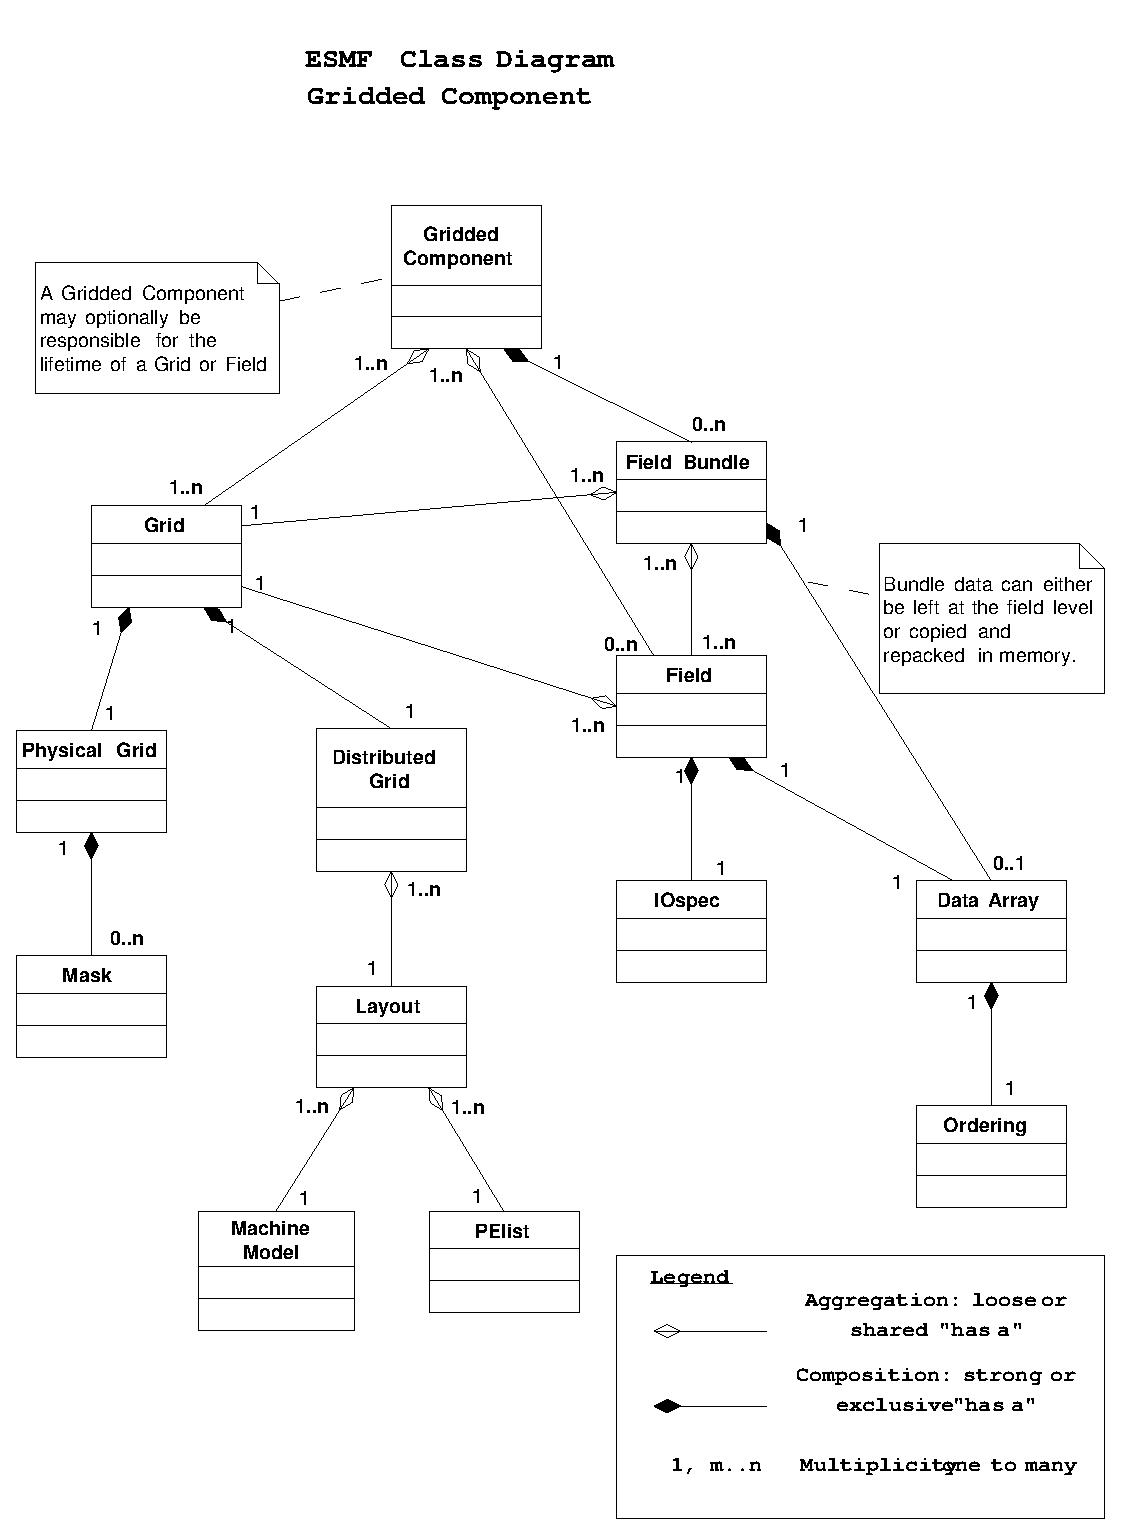
\includegraphics{ESMF_DataStructureHierarchy.eps}}


\subsubsection{Bundle (ESMF\_Bundle)}
\label{sec:bundle} 
\begin{description}
\item [Description] A Bundle contains one or more Fields which are defined on 
the same Grid.  It allows the application to manipulate multiple fields in 
an identical manner with a single set of calls.  It also allows the option 
of interleaving data from multiple fields into a single Data Array for 
more efficient memory access patterns.  
\item [Function] The Bundle class is an aggregation of the Field class.  
It provides methods for getting and setting fields.  It provides methods 
for querying information about the
underlying grid.  It provides methods for requesting the packing of data, the
reordering of that packed data, and detaching and attaching the data.
\end{description}


\subsubsection{Field (ESMF\_Field)}
\label{sec:field} 
\begin{description} 
\item [Description] A Field represents a single physical field or the components of a 
vector field.  It is the basic data carrying object in the system.  It includes both
the data and the grid on which the data are defined.  The main application interfaces
for accessing data are here.
\item [Function] The Field object is a composition of the Data Array object,
an optional IOspec object, and it aggregates a Grid object.  It provides
methods for getting, setting, and querying the data array, the grid, the mask and
the I/O spec.  It provides methods for detaching and attaching data from the field.
While data are detached it is the responsibility of the application.  A Field object
provides methods for subsetting, regridding, and reordering memory layout of data.
\end{description}

\subsubsection{Mask (ESMF\_Mask)}
\label{sec:mask} 
\begin{description}
\item [Description] A Mask describes a subset of data items, for example to indicate
the valid values which represent ocean points (and not land) in an ocean model.  
It may be specified at the Field object level, but it is stored as part of the PhysGrid object.
\item [Function] The Mask class is an optional part of a PhysGrid class.  
It provides methods for getting and setting valid values.
\end{description}

\subsubsection{Data Array (ESMF\_Data)}
\label{sec:dataarray} 
\begin{description}
\item [Description] A Data Array is a list of data values plus information about
the data values.
\item [Function] The Data class contains the data as well as information 
about the data, including the data type (e.g. float,
integer), the machine type (e.g. IEEE float, Cray float), 
data count, data dimensionality (e.g. scalar, vector).  
It provides methods for querying information about the data,
returning a pointer to the memory location of the start of the data, 
and conversion routines for altering the characteristics of the data.  
Information about how the data array is laid
out in memory is managed by the Ordering class.

Data Arrays can contain either homogeneous or composite data types 
(e.g records or structures).
Data Arrays can be associated with a Field object or with a Bundle object.
Data associated with a Field object consist of only a single variable.  
Data associated
with a Bundle object can have data from multiple Fields packed into a single
buffer with the items interleaved in memory.  
The application may use a packed array to increase
locality of reference while iterating the array, 
or for ease in subsetting multiple data values in one operation.
Information about the multi-field packing and methods to reorder the
data are managed by the Ordering class.

\end{description}

\subsubsection{Ordering (ESMF\_Ordering)}
\label{sec:ordering} 
\begin{description}
\item [Description] A Ordering is the description of how multidimentional data have been
linearized in memory.  This includes multidimensional array index information (e.g. C-order
vs Fortran-order), vector or tensor data item ordering information (e.g. all Xs then all
Ys vs [X,Y], [X,Y] tuples), and for Arrays associated with a Bundle object which contain
data for multiple fields, interleave information about how multiple field data are 
packed into a single buffer.
\item [Function] An Ordering object is associated with a single Data object.  It provides
methods to query the current memory organization and methods to reorder the Data object.
\end{description}

\subsubsection{Grid (ESMF\_Grid)}
\label{sec:ordering} 
\begin{description}
\item [Description] A Grid is the general representation of the coordinate information for
the computation.  It contains both the logical presentation of the grid as well as the
decomposition of the grid into subgrids for processing in parallel on a
multiprocessor system.
\item [Function] The Grid class is the composition of a PhysGrid and a DistGrid object.  
It is aggregated into the Field and the Bundle objects.  It provides methods to the
Field and Bundle classes for obtaining coordinate, indexing, and decomposition information.
\end{description}

\subsubsection{Physical Grid (ESMF\_PhysGrid)}
\label{sec:physgrid} 
\begin{description}
\item [Description] A Physical Grid is a discrete representation of a continuous physical space.
There are a multitude of types of physical grids.
The grid contains the physical coordinates, usually indicating where data values are located, but
it could also be a parametric description of the actual locations.  
\item [Function] The PhysGrid class maintains a global index space for coordinate information.
It provides methods for creating a variety of grid types, including both reading grid information
and generating grids from parameters.  It provides methods for regridding, or translating
one grid to another, used for example when exchanging data through the coupler between
various components.
The PhysGrid class does not handle grid decomposition issues related to 
distributed processing; see the Distributed Grid object in Section~\ref{distgrid}.
\end{description}

\subsubsection{Distributed Grid (ESMF\_DistGrid)} 
\label{sec:distgrid} 
\begin{description}
\item [Description] A Distributed Grid is a collection of subgrids which
constitute a single logical grid.  The subgrids can be operated on in
parallel on a multiple processor machine.  
\item [Function] The DistGrid class contains the mapping
between the local grid decompositions and the global logical grid. 
It contains methods to 
synchronize data values between the boundaries of subsets, and to
collect and communicate global data values.  It interacts closely with
the Physical Grid object (see Section~\ref{physgrid}).
It uses a Layout object to identify and manage the processing elements 
available for the computation.
\end{description}

\subsubsection{Input/Output Specfication (ESMF\_IOspec)}
\label{sec:iospec} 
\begin{description}
\item [Description] A Input/Output specfication contains all 
information necessary to read or write objects.  It includes the 
destination information (e.g. file, socket), the name,
the format, and any additional parameters needed to complete the I/O.
\item [Function] The IOspec class provides a format-independent layer by
providing generic methods such as Initialize/Finalize, Open/Close, 
and Read/Write which are not specific to any one input or output format.
The methods
within the IO layer will encapsulate format dependent parameters and calls.
The IO layer will write not only the simulation output (large, computational
data) but also the metadata which is required to document what the data is
and information about how it was generated.
The ESMF library will probably strive simply to
support the existing variety of file formats which are in common use in
the climate community, but looking forward
the existence of this class lays the foundation for future extension 
of IO beyond simple files to live connections to database systems, 
web servers, etc.
\end{description}




